\section{Auswertung}
\label{sec:Auswertung}

Im ersten Schritt soll eine Gaußverteilung  an den Detektor-Scan gefittet und die Werte der maximalen Intensität und der Halbwertsbreite ermittelt werden.
Die Daten und der Fit einer Gaußfunktion an die Daten nach der Formel 
\begin{equation*}
    I(\theta) = \frac{a}{\sigma\sqrt{2\pi}} \exp\left( \frac{-\left( \theta - \theta_0\right)^2}{2 \sigma} \right)
\end{equation*} sind in Abbildung \ref{abb:detector} zu sehen.
Die Werte, die sich aus dem Fit ergeben sind
\begin{align*}
a &= \num{1.815(15)e5} \\
\theta_0 &= \SI{0.0018(4)}{\degree} , \\
\sigma &= \SI{0.0418(4)}{\degree}\,. \\
\end{align*}

Die Amplitude $ \frac{a}{\sigma\sqrt{2\pi}}$ ergibt sich somit zu \num{1.732(22)e6} Events als Maximum. 
Die Halbwertsbreite beträgt $2 \sqrt{2 \ln 2} \, \sigma$, also \SI{0.0985(9)}{\degree}.
\begin{figure}
    \centering
    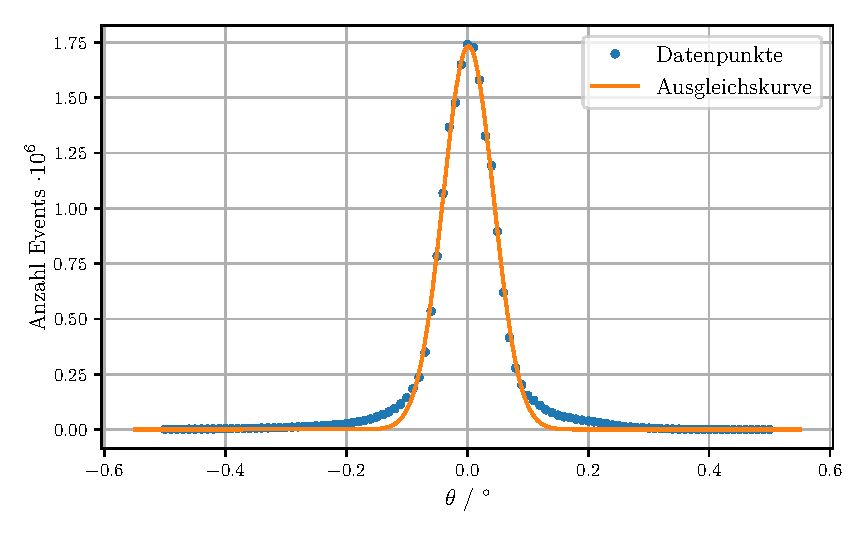
\includegraphics[width=0.8\textwidth]{figures/detector_scan.pdf}
    \caption{Die gemessenen Daten des Detektor-Scans und eine an die Daten gefittete Gaußverteilung sind hier abgebildet.}
    \label{abb:detector}
\end{figure}

Die Reflektivität ergibt sich aus der Differenz des diffusen Scan und der eigentlichen Messwerten. 
Die korrigierten Werte sind gemeinsam mit dem diffusen Scan und den Messwerten in Abbildung \ref{abb:diffus} zu sehen.

\begin{figure}
    \centering
    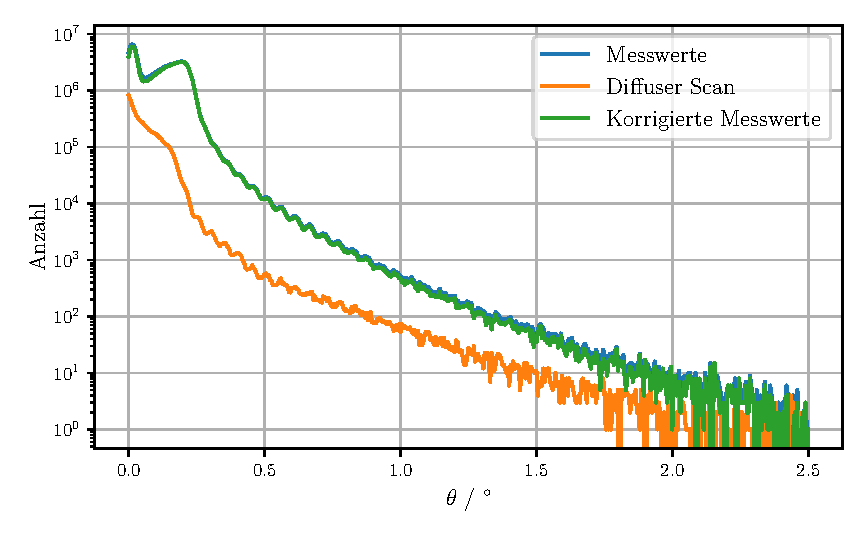
\includegraphics[width=0.8\textwidth]{figures/messwerte_relativ.pdf}
    \caption{Die korrigierten Werte, die sich als Differenz aus den Messwerten und dem diffusen Scan ergeben, sind hier gezeigt.}
    \label{abb:diffus}
\end{figure}

Anschließend werden die Werte am Winkel des Maximums \SI{0.195}{\degree} normiert und neben der Theoriekurve der Fresnelreflektivität einer idealen glatten Siliciumoberfläche, die sich aus Formel \eqref{eq:r} ergibt, in Abbildung \ref{abb:norm} aufgetragen. Der dafür benötigte Wellenvektor ergibt sich über die Wellenlänge der K-$\alpha$ Linie von Kupfer mit einem Wert von $\lambda = \SI{1.54e-10}{\meter}$. 
Der benötigte Brechungsindex von Silicium ist $n = \num{1} - \num{7.6e-6} + \num{1.73i e-9}$ \cite{skript}.
\begin{figure}
    \centering
    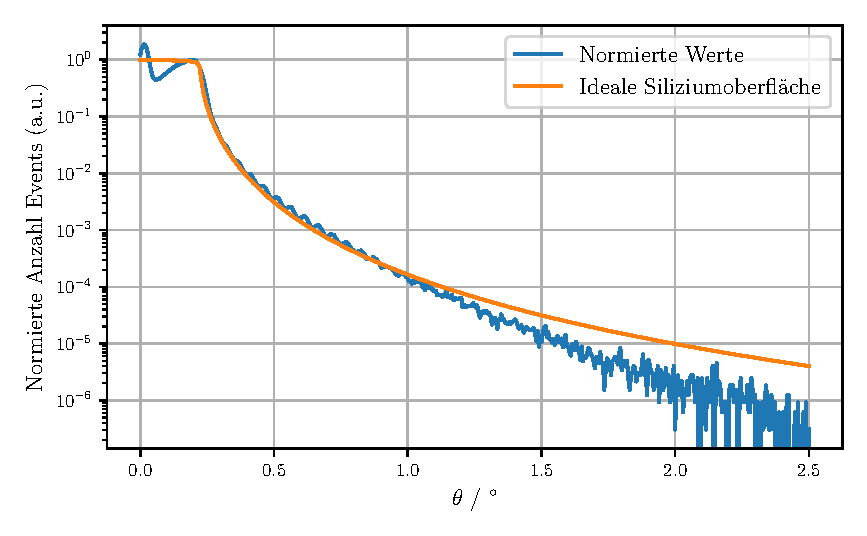
\includegraphics[width=0.75\textwidth]{figures/messwerte_norm.pdf}
    \caption{Normierte Messwerte und die Theoriekurve der Fresnelreflektivität einer glatten Siliciumoberfläche.}
    \label{abb:norm}
\end{figure}

Der Geometriewinkel lässt sich aus Abbildung \ref{abb:dreieck} ablesen. 
Der Abstand von der Mitte bei $\theta = \SI{0}{\degree}$ zu den Schnittpunkten des Dreiecks entspricht dem Wert des Geometriewinkels. 
Dieser beträgt $\theta_g = \SI{0.7}{\degree}$. 
Mithilfe der Formel \eqref{eq:geometrie} und dem gemessenen Durchmesser der Probe, der $D = \SI{21.5}{\milli\metre}$ beträgt, ergibt sich die Strahlhöhe $d_0 = \SI{0.263}{\milli\meter}$ und ein Geometriefaktor von $G = \num{81.85} \cdot \sin \theta_i$ für alle Winkel $\theta_i$ die kleiner als der Geometriewinkel $\theta_g$ sind.

\begin{figure}
    \centering
    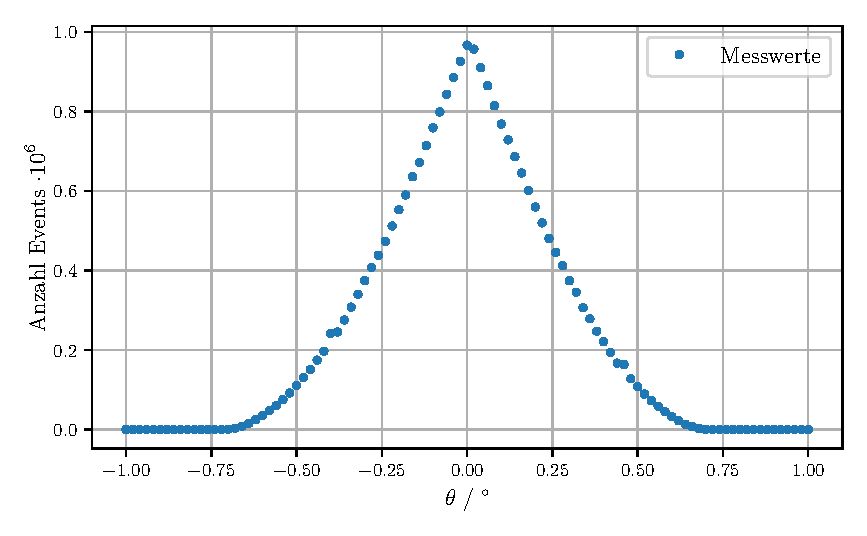
\includegraphics[width=0.75\textwidth]{figures/dreieck.pdf}
    \caption{Hier sind die Messwerte des Rocking-Scan während der Justage aufgetragen.}
    \label{abb:dreieck}
\end{figure}

Aus den Kiessig-Oszillationen ergibt sich nach Gleichung \eqref{eq:kiessig} die Schichtdicke. 
Dafür müssen die Stellen der Minima bestimmt werden. 
Hier wurden 8 eindeutige Minima gemessen. Aus den Positionen dieser Minima lässt sich dann der Betrag der Wellenvektorüberträge $q$ bestimmen und aus der Differenz dieser Werte ergibt sich dann die Schichtdicke $z$. Diese beträgt im Mittel $z = \SI{876(30)}{\angstrom}$. Die entsprechenden Werte der einzelnen Minima sind in Tab. \ref{tab:kiessig} aufgetragen. 

\begin{table} \caption{Die Stellen der Minima, die Beträge der Wellenvektorüberträge $q$ und die Differenzen dieser Werte sind hier zusammen mit den resultierenden Schichtdicken aufgelistet.}
    \label{tab:kiessig}
    \centering
    \sisetup{round-mode =places, round-integer-to-decimal=true, round-precision=3}
    \begin{tabular}{S[] S[] S[] S[]}
        \toprule
        {$\theta_i / \si{\degree}$} & {$q_i / 10^8 \si{\meter}$} & {$q_{i+1} - q_{i}/ 10^8 \si{\meter}$} & {$z / \si{\angstrom}$} \\
        \midrule
        0.400 & 5.697  &   0.641 & 980.421  \\
        0.445 & 6.338  &   0.712 & 882.385  \\
        0.495 & 7.050  &   0.641 & 980.434  \\
        0.540 & 7.690  &   0.783 & 802.180  \\
        0.595 & 8.474  &   0.712 & 882.407  \\
        0.645 & 9.186  &   0.783 & 802.196  \\
        0.700 & 9.969  &   0.783 & 802.206  \\
        0.755 & 10.752 &         &          \\
        \bottomrule
    \end{tabular}
\end{table}

Zur Bestimmung des Dispersionsprofils wird der Parratt-Algorithmus benutzt. 
In Abbildung \ref{abb:parratt} sind die Messwerte zusammen mit einer Theoriekure des Parratt-Algorithmus aufgetragen. 
Als Parameter wurden hierbei nach Formel \eqref{eq:imag} und \eqref{eq:rau} die Werte in Tabelle \ref{tab:parratt} genutzt. 
Der entsprechende Code befindet sich im Anhang in Kapitel \ref{sec:Anhang}.
In der Theoriekurve passt $z = \SI{8.2}{\angstrom}$ am besten. 

\begin{table} \caption{Die Parameter, die für den Parratt Algorithmus genutzt wurden. Dabei ist jeweils der Name des Materials, die Dispersion $\delta$, das Produkt aus Wellenlänge und Absorptionskoeffizient $\beta = \frac{\lambda}{4 \pi} \cdot \mu$ und die Faktoren $\sigma$, die die Rauigkeit in den modifizierten Fresnelkoeffizienten beschreiben.}
    \label{tab:parratt}
    \centering
    %\sisetup{round-mode =places, round-integer-to-decimal=true, round-precision=3}
    \begin{tabular}{c S[] S[] S[]}
        \toprule
        {Probe} & {$\delta / 10^{-6}$} & {$\beta / 10^{-7}$} & {$\sigma / 10^{-10}$} \\
        \midrule
        Silicium   & 5.7 & 6.13 & 8.0 \\
        Polystyrol & 5.1 & 4.9  & 5.5 \\
        \bottomrule
    \end{tabular}
\end{table}


\begin{figure}
    \centering
    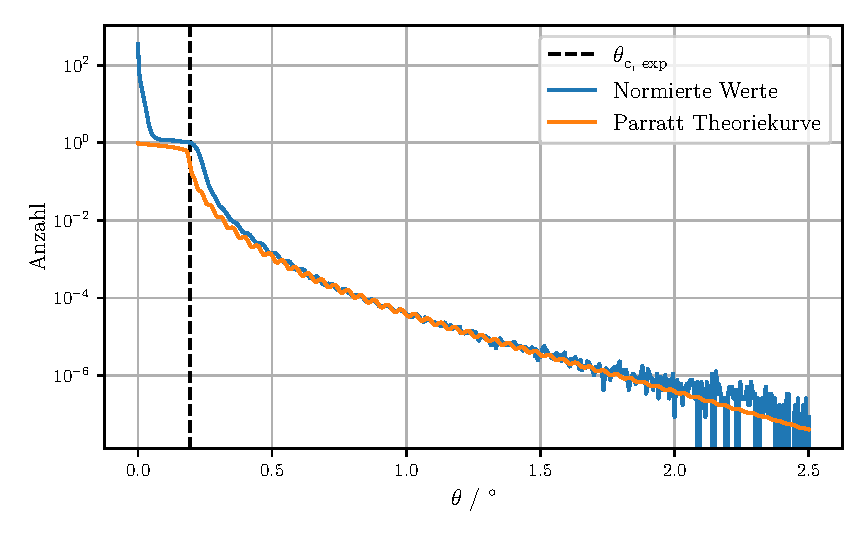
\includegraphics[width=\textwidth]{figures/parat.pdf}
    \caption{Hier sind die normierten Messwerte und eine Theoriekurve des Parratt-Algorithmus.}
    \label{abb:parratt}
\end{figure}

Aufgrund der Formel \eqref{eq:delta} ergibt sich aus den $\delta$-Werten der Theoriekurve ein kritischer Winkel von $\theta_\text{c, Parratt, Si}= \SI{0.193}{\degree}$ und $\theta_\text{c, Parratt, PS}= \SI{0.183}{\degree}$. Die Literaturwerte aus Referenz \cite{skript} sind $\theta_\text{c, Lit, Si}= \SI{0.223}{\degree}$ und $\theta_\text{c, Lit, PS}= \SI{0.153}{\degree}$. 
Der Wert, der sich hier bei der Kurve ablesen lässt, liegt bei ca. $\theta_\text{c, exp}= \SI{0.195}{\degree}$.

